% mnras_template.tex 
%
% LaTeX template for creating an MNRAS paper
%
% v3.0 released 14 May 2015
% (version numbers match those of mnras.cls)
%
% Copyright (C) Royal Astronomical Society 2015
% Authors:
% Keith T. Smith (Royal Astronomical Society)

% Change log
%
% v3.0 May 2015
%    Renamed to match the new package name
%    Version number matches mnras.cls
%    A few minor tweaks to wording
% v1.0 September 2013
%    Beta testing only - never publicly released
%    First version: a simple (ish) template for creating an MNRAS paper

%%%%%%%%%%%%%%%%%%%%%%%%%%%%%%%%%%%%%%%%%%%%%%%%%%
% Basic setup. Most papers should leave these options alone.
\documentclass[fleqn,usenatbib]{mnras}

% MNRAS is set in Times font. If you don't have this installed (most LaTeX
% installations will be fine) or prefer the old Computer Modern fonts, comment
% out the following line
\usepackage{newtxtext,newtxmath}
% Depending on your LaTeX fonts installation, you might get better results with one of these:
%\usepackage{mathptmx}
%\usepackage{txfonts}

% Use vector fonts, so it zooms properly in on-screen viewing software
% Don't change these lines unless you know what you are doing
\usepackage[T1]{fontenc}
\usepackage{ae,aecompl}




%%%%% AUTHORS - PLACE YOUR OWN PACKAGES HERE %%%%%

% Only include extra packages if you really need them. Common packages are:
\usepackage{graphicx}	% Including figure files
\usepackage{amsmath}	% Advanced maths commands
\usepackage{amssymb}	% Extra maths symbols
\usepackage{siunitx} %v. useful units package 

%%%%%%%%%%%%%%%%%%%%%%%%%%%%%%%%%%%%%%%%%%%%%%%%%%

%%%%% AUTHORS - PLACE YOUR OWN COMMANDS HERE %%%%%

% Please keep new commands to a minimum, and use \newcommand not \def to avoid
% overwriting existing commands. Example:
%\newcommand{\pcm}{\,cm$^{-2}$}	% per cm-squared
\newcommand{\xip}{\ensuremath{\xi_{+}}}
\newcommand{\xim}{\ensuremath{\xi_{-}}}
\newcommand{\xipm}{\ensuremath{\xi_{\pm}}}
\newcommand{\gammat}{\ensuremath{\gamma_{t}(\theta)}}
\newcommand{\wtheta}{\ensuremath{w(\theta)}}
\newcommand{\dsigr}{\ensuremath{\Delta\Sigma(R)}}
\newcommand{\dsigobsr}{\ensuremath{\Delta\Sigma^{\mathrm{obs}}(R)}}
\newcommand{\dsigmodr}{\ensuremath{\Delta\Sigma^{\mathrm{model}}(R)}}

\newcommand{\pgg}{\ensuremath{P_{\mathrm{gg}}}}
\newcommand{\pgm}{\ensuremath{P_{\mathrm{gm}}}}
\newcommand{\xigg}{\ensuremath{\xi_{\mathrm{gg}}}}
\newcommand{\xigm}{\ensuremath{\xi_{\mathrm{gm}}}}

%units
\DeclareSIUnit \megaparsec {Mpc}
\DeclareSIUnit \h {\mbox{$h$}}

%cosmo parameters
\newcommand{\om}{\ensuremath{\Omega_{\mathrm m}}}
\newcommand{\ol}{\Omega_{\mathrm \Lambda}}
\newcommand{\omb}{\Omega_{\mathrm b}}
\newcommand{\sig}{\ensuremath{\sigma_8}}
\newcommand{\lcdm}{$\Lambda$CDM}
\newcommand{\wcdm}{$w$CDM}
\newcommand{\ns}{n_s}
\newcommand{\w}{w_0}
\newcommand{\wa}{w_a}

% eqn and figures
\newcommand\eqn[1]{equation~\ref{#1}}
\newcommand\eqnb[2]{equations~\ref{#1}~\& \ref{#2}}
\newcommand\eqnc[2]{equations~\ref{#1}--\ref{#2}}
\newcommand\Eqn[1]{Equation~\ref{#1}}   % If you need to start a sentence with this...
\newcommand\Eqnb[2]{Equations~\ref{#1}~\& \ref{#2}}

% Likewise for figures and tables
\newcommand\fig[1]{Figure~\ref{#1}}
\newcommand\figb[2]{Figures~\ref{#1}~\& \ref{#2}}
\newcommand\chap[1]{Chapter~\ref{#1}}
\newcommand\sect[1]{Section~\ref{#1}}
\newcommand\tab[1]{Table~\ref{#1}}
\newcommand\app[1]{Appendix~\ref{#1}}
\newcommand{\redmagic}{\texttt{redMaGiC}\,}
\newcommand{\mice}{\texttt{MICE}\,}
\newcommand{\maglim}{\texttt{Maglim}\,}
\newcommand{\buzzard}{\texttt{Buzzard}\,}

\newcommand{\SP}[1]{{\color{brown}[SP: #1]}}

%%%%%%%%%%%%%%%%%%%%%%%%%%%%%%%%%%%%%%%%%%%%%%%%%%

%%%%%%%%%%%%%%%%%%% TITLE PAGE %%%%%%%%%%%%%%%%%%%

% Title of the paper, and the short title which is used in the headers.
% Keep the title short and informative.
\title[Short title, max. 45 characters]{DES Y3 results: Constraints on cosmological parameters and galaxy bias models from galaxy clustering and galaxy-galaxy lensing}

% The list of authors, and the short list which is used in the headers.
% If you need two or more lines of authors, add an extra line using \newauthor
\author[DES et al.]{
DES
}

% These dates will be filled out by the publisher
\date{Accepted XXX. Received YYY; in original form ZZZ}

% Enter the current year, for the copyright statements etc.
\pubyear{2015}

% Don't change these lines
\begin{document}
\label{firstpage}
\pagerange{\pageref{firstpage}--\pageref{lastpage}}
\maketitle

% Abstract of the paper
\begin{abstract}
We present cosmological constraints from the combination of galaxy clustering and galaxy-galaxy lensing measurements from the DES Y3 data. We describe our modeling framework and choice of scales, validating their robustness to small-scale theoretical uncertainties by analysing simulated data. We implement nonlinear bias models that include parameterizations based on Lagrangian perturbation theory. We present cosmological constraints when using various (coupled) choices of scale cuts and bias models and demonstrate stability of the constraints. We reproduce the baseline choices of the 3x2 cosmology paper, and consider additional choices that make use of small scale information.  Combining with external datasets including Planck, we show constraints on w, as well as higher order galaxy bias parameters
\end{abstract}

% Select between one and six entries from the list of approved keywords.
% Don't make up new ones.
\begin{keywords}
keyword1 -- keyword2 -- keyword3
\end{keywords}

%%%%%%%%%%%%%%%%%%%%%%%%%%%%%%%%%%%%%%%%%%%%%%%%%%

%%%%%%%%%%%%%%%%% BODY OF PAPER %%%%%%%%%%%%%%%%%%

\section{Introduction}

\begin{itemize}
    \item LSS can tell us about dark energy.
    \item Galaxy clustering and galaxy-galaxy lensing is a good combo for probing LSS.
    \item Modeling galaxy bias is the main theoretical challenge for this.
\end{itemize}

\section{Statistics and theory}

\subsection{Two-point statistics}

\begin{itemize}
    \item Describe the statistics we use, \wtheta\ and \gammat.
    \item Show their relation to the underlying 3d correlation functions $\xigg(r)$ and $\xigm(r)$
\end{itemize}

\brown{Using the catalog of the positions of foreground lens galaxies and the catalog of shape and positions of background source galaxies, one can construct three two point summary statistics. The two point auto-correlation of the positions of lens galaxies (galaxy clustering), auto-correlation of the lensing shear estimated from shape of background source galaxies (cosmic shear) and  cross-correlation of this lensing shear field and position of lens galaxies (galaxy-galaxy lensing). 

For the galaxy clustering we use the $w(\theta)$ statistic which quantifies the average excess number of galaxy pairs at a separation $\theta$ over a random distribution. For galaxy-galaxy lensing, we use the statistic of $\gamma_{\rm t}(\theta)$ that describes the average tangential component of the shear with respect to the lens-source separation direction. For cosmic shear, which is a spin-2 field, we use the statistic of $\xi_{+}$ and $\xi_{-}$. 




}


\subsection{P(k) predictions}
\begin{itemize}
    \item Heavily referencing Shivam's paper, describe range of perturbation theory models for $\xigg(r)$ and $\xigm(r)$ and their expected scales of applicability. 
    \item To aid discussion, include some plots showing the sensitivity of our statistics to scales in $\xigg(r)$ and $\xigm(r)$.
    
    \brown{As we saw in the previous section, the statistics of our main interest here $w(\theta)$ and $\gammat$ is related to the underlying 3D correlation functions \xigg and \xigm respectively. 
    
    }
    
\end{itemize}

\subsection{The rest of the model}
Describe the rest of the modelling framework:
\begin{itemize}
    \item IAs (NLA)\brown{TATT?}
    \brown{Galaxy galaxy lensing aims to isolate the percent-level coherent shape distortions, or shear, of background source galaxies due to graviataional field of foreground lens galaxies. However, the local environment can align the source galaxies as well as also contribute to the shear signal through lensing distortions. Since this interaction between the source galaxies and their local environment is non-random, it has non-zero contribution to the galaxy-galaxy lensing signal which we need to model. In this analysis we follow the mixed alignment methodolgy of \cite{Blazek_2019}. }
    \item Magnification
    \brown{All the matter between observed galaxy and the observer acts as a gravitational lens. Hence the galaxies get magnified which results in an increase in the size of galaxy images as well as increase in their total flux. The increase in the size of galaxies results in decrease in observed number density (due to stretching of local sky), whereas due to increase in total flux results in increase in number density (as intrinsically fainter galaxies, which are more numerous, can be observed).  }
    \item RSD
    \brown{}
\end{itemize}    

    
    \SP{
    \begin{itemize}
    \item Point-mass marginalization 
    \item  Motivate that we will be using the $\Sigma^{-1}_{\rm crit}$ factors when doing the PM marginalization. 
    \item \textbf{\textit{Figure}} Plot comparing the contours with vs without PM marginalization for both 2x2pt and 3x2pt. Make (or show) the argument that it is because of breaking of degeneracy between PM and S8. Basically make the case that PM does not matter for 3x2pt and that 2x2pt can have more aggressive scale cuts than 3x2pt analysis.
    \end{itemize}
    }
    
        
    \brown{The galaxy-galaxy lensing signal is related to the mass density of lenses by:
    \begin{equation}
        \gamma_{\rm t}(R;z_{\rm l},z_{\rm s}) = \frac{\Delta \Sigma (R;z_{\rm l})}{\Sigma_{\rm crit} (z_{\rm l},z_{\rm s})},
    \end{equation}
    where, $\Delta \Sigma(R;z_{\rm l}) = \bar{\Sigma}(0,R; z_{\rm l}) - \Sigma(R;z_{\rm l})$ and $\Sigma(R;z_{\rm l})$ is the surface mass density at a transverse separation $R$ from the lens at redshift $z_{\rm l}$ and $\bar{\Sigma}(0,R)$ is the average surface mass density within a separation $R$ from that lens. Through $\bar{\Sigma}(0,R)$ term, $\gamma_{\rm t}$  at any scale $R$, is dependent on mass distribution at all scales less than $R$. This makes $\gamma_{\rm t}$ statistic highly non-local and any model that is valid only on large scales above some $r_{\rm min}$ (like PT) will break down more rapidly than for a more local statistic like \wtheta. However, as the dependence on small scales is through the \textit{mean} surface mass density, the impact of mass distribution inside $r_{\rm min}$ on \gammat can be written as:
    \begin{equation}
        \gamma_{\rm t}(R;z_{\rm l},z_{\rm s}) = \frac{1}{\Sigma_{\rm crit}(z_{\rm l},z_{\rm s})} \bigg(\Delta \Sigma^{\rm model}(z_{\rm l}) + \frac{B(z_{\rm l})}{R^2} \bigg),
    \end{equation}
    where, $\Delta \Sigma^{\rm model}$ is the prediction from a model that is valid of scales above $r_{\rm min}$ and $B$ is the effective total mass below $r_{\rm min}$.  The average $\gamma_{\rm t}$ signal between lens bin $i$ and source bin $j$ can be written as:
    \begin{equation}
        \gamma_{{\rm t},ij} = \gamma^{\rm model}_{{\rm t},ij} + C_{ij}/\theta^2,
    \end{equation}
    where,
    
    \begin{equation}\label{eq:pm_Cij}
        C_{ij} = \int dz_{\rm l} \ dz_{\rm s} \ n_{{\rm l},i} \ n_{{\rm s},j} \ B_i(z_{\rm l}) \ \Sigma^{-1}_{\rm crit}(z_{\rm l},z_{\rm s}) \ \chi^{-2}(z_{\rm l}).
    \end{equation}
    Here $B_i$ is the PM for lens bin $i$, $n_{{\rm l},i}$ is the redshift distribution of lenses for tomographic bin $i$, $n_{{\rm s},j}$ is the redshift distribution of sources for tomographic bin $j$ and $chi(z_{\rm l})$ is the comoving distance to lens redshift $z_{\rm l}$. We find that for tomographic bins of our lens sample, we can make the approximation that PM evolves slowly with redshift and hence take $B_i$ out of the double integral in Eq.~\ref{eq:pm_Cij}. Therefore, in our fiducial analysis, we treat the parameters $B_i$ as a constant to marginalize over for any lens bin $i$ and is independent of the redshift distribution of sources. 
    }
    
    \begin{figure}
    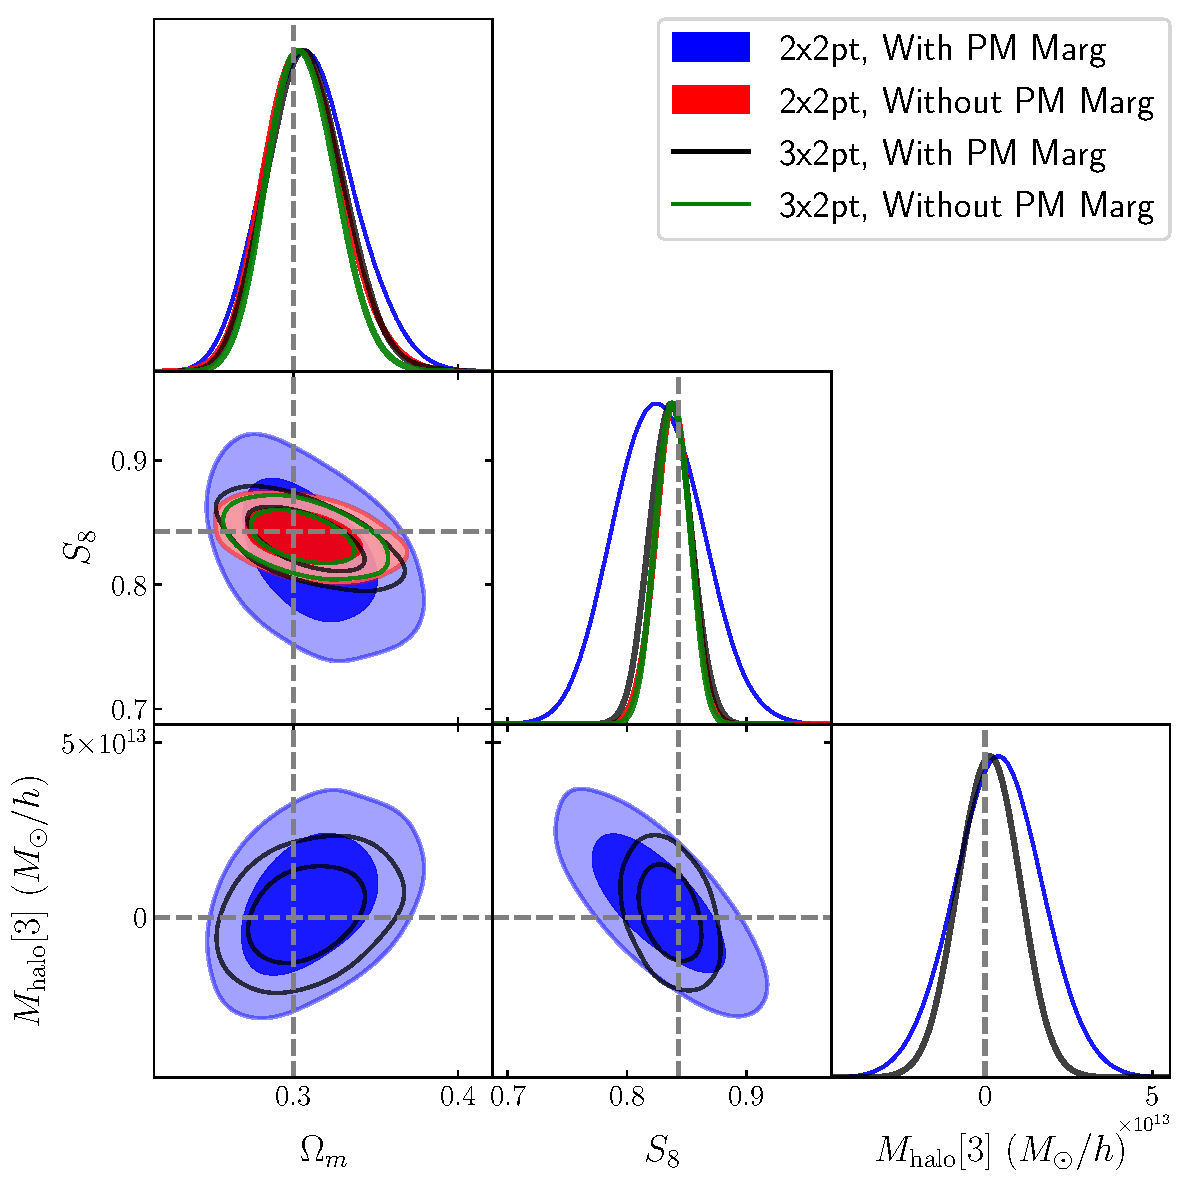
\includegraphics[width=\columnwidth]{figs/compare_cosmo_pm_marg_2x2pt_3x2pt_fullspace.pdf}
    \caption[]{Effect of point mass marginalization on the constraining power of 2x2pt and 3x2pt. We see that the constraining power of 2x2pt degrades significantly with point mass marginalization, while for 3x2pt the change is minimal. Including the shear-shear correlation information breaks the degeneracy between point-mass (we show PM for third bin, $M_{\rm halo}[3]$) and $S_8$, leading to smaller sensitivity of cosmology constraints on point mass constraints. }
    \label{fig:pm_effect}
    \end{figure}
\begin{itemize}
    \item Shear-ratio information
    \brown{As we are using }
    \item projection of $P(k)$s to $C_l$ and conversion of $C_l$s to $w(\theta),\gamma_t(\theta)$.
\end{itemize}

% \begin{figure}
% \includegraphics[width=\columnwidth]{figs/pm_evolution.png}
% \caption[]{ Evolution galaxy correlation function across the first redshift bin and its contribution to PM till 6Mpc/$h$.  }
% \label{fig:pm_evolve}
% \end{figure}


\section{The datavector}
We describe the Y3 2x2pt datavector (and it's input data).

\section{Validation of parameter inference}

\subsection{Models, scale cuts, priors and external datasets}
We describe the models, scale cuts, priors and external datasets we'll use.

\subsubsection{DES 2 $\times$ 2pt models + priors}
For DES 2x2pt, we test 3 different galaxy bias model + prior choices:
\begin{enumerate}
    \item Linear bias
    \item 1-loop with a free $-5<b_2<5$ for each lens bin, and $b_s, b_{3nl}$ fixed to co-evolution Lagrangian values.
    \item Free $-5<b_2<5, -5<b_s<5, -5<b_{3nl}<5$ ($b_k$?).
\end{enumerate}

\subsubsection{Scale cuts}
Motivated by Shivam's bias modelling paper, we choose 2 or 3 sets of scale cuts.

\subsection{Cosmological models, external datasets and priors}
We test the following cosmological model and prior combinations
\begin{enumerate}
    \item Flat \lcdm\ with uninformative priors
    \item Flat \lcdm\ with informative priors on some combination of $\Omega_m$, $H_0$ and $n_s$ TBD.
    \item Flat \wcdm 
    \item Flat \wcdm\ with Planck.
\end{enumerate}

\subsection{Simulated Likelihood tests}

We perform simulated likelihood tests to reveal which of our analysis choice combinations (i.e. scale cuts + bias model + priors + external dataset + cosmological model) return unbiased cosmological parameters.

\brown{In this section we analyze linear bias model using a simulated datavector having contamination from higher order non-linearities. We simulate a datavector which receives contribution from non-linear bias and baryonic physics. For non-linear bias, we use the bestfit $b_1$ and $b_2$, as esitmated from 3D analysis of \mice simulation.  }

\SP{\begin{itemize}
    \item \textbf{\textit{Figure}} Linear bias recovering unbiased cosmology (for $\Lambda$CDM) at Scale Cut (X,Y) Mpc/$h$. Show contours also for one scale cut smaller and one scale cut bigger than this. 
    \item \textbf{\textit{Figure}} Linear bias $w$CDM: Show results for $w$CDM with and without Planck
    \item \textbf{\textit{Figure}} Non-linear bias $\Lambda$CDM: Show the results for non-linear bias LCDM recovering true cosmology when the input bs and b3nl are not given by co-evolution relation but model uses those relations.
\end{itemize}
}

\begin{figure*}
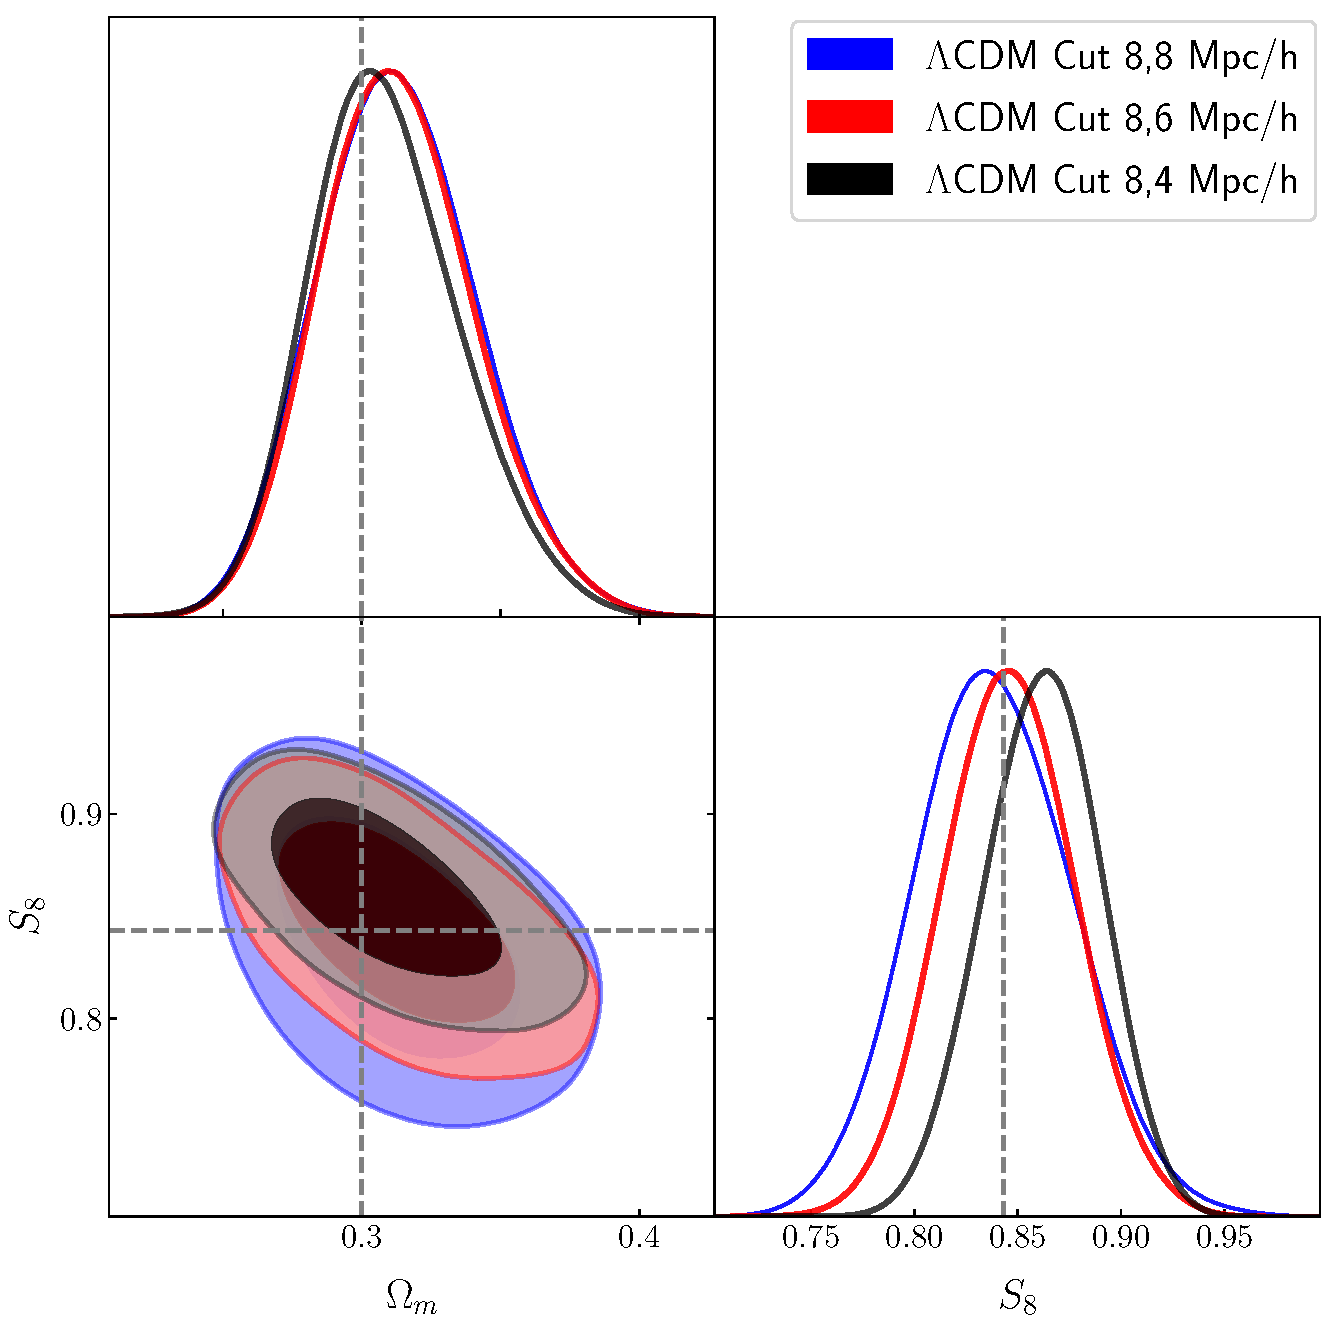
\includegraphics[width=\columnwidth]{figs/compare_cosmo_lcdm_8_8-6-4_simple.pdf}
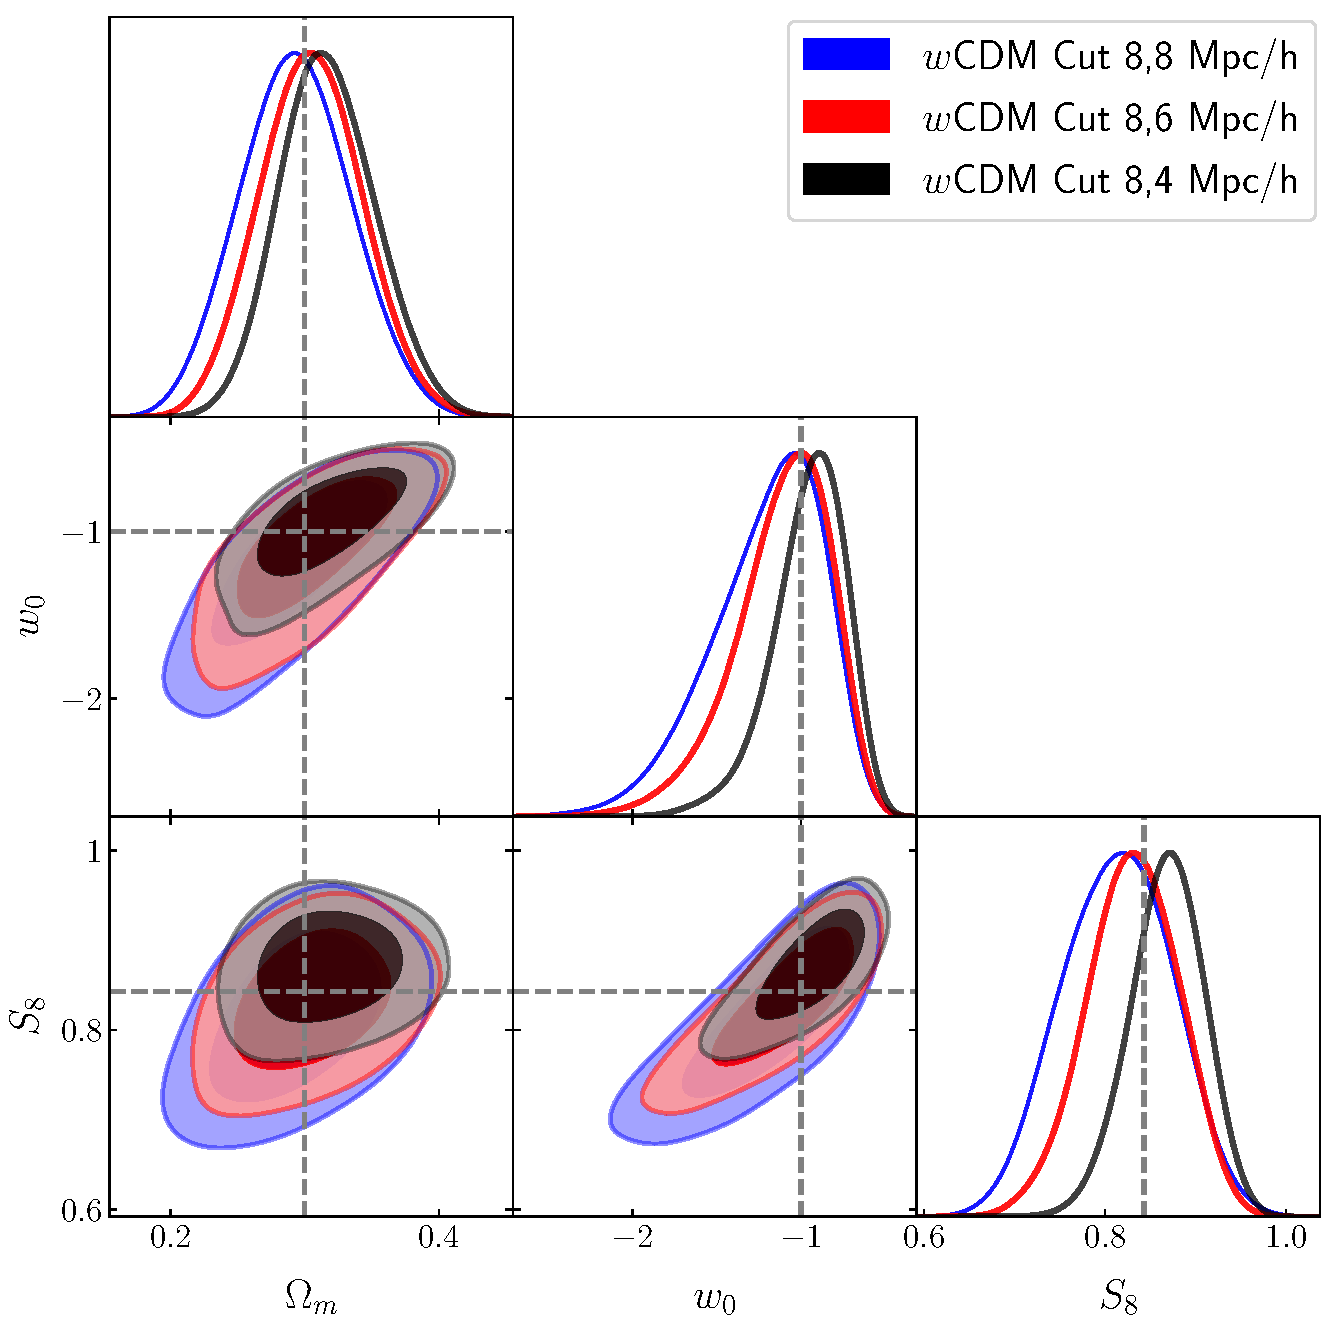
\includegraphics[width=\columnwidth]{figs/compare_cosmo_wcdm_8_8-6-4_simple.pdf}
\caption[]{\lcdm\ Simulated likelihood analysis when analyzing a datavector contaminated with non-linear bias + baryons and analyzed with linear bias + halofit as model. We see that we get unbiased cosmology with a scale cut of (8,6)Mpc/$h$ for both \lcdm and $w$CDM cosmology. }
\label{fig:sim_lin}
\end{figure*}

\subsection{Results on Buzzard simulations}

For those analysis choice combos passing the simulated likelihood tests, we validate on the suite of Y3 buzzard simuulations. Select analysis choice combinations that return unbiased cosmological parameters to run on the data. 

\subsubsection{DES-only \lcdm}

\begin{figure*}
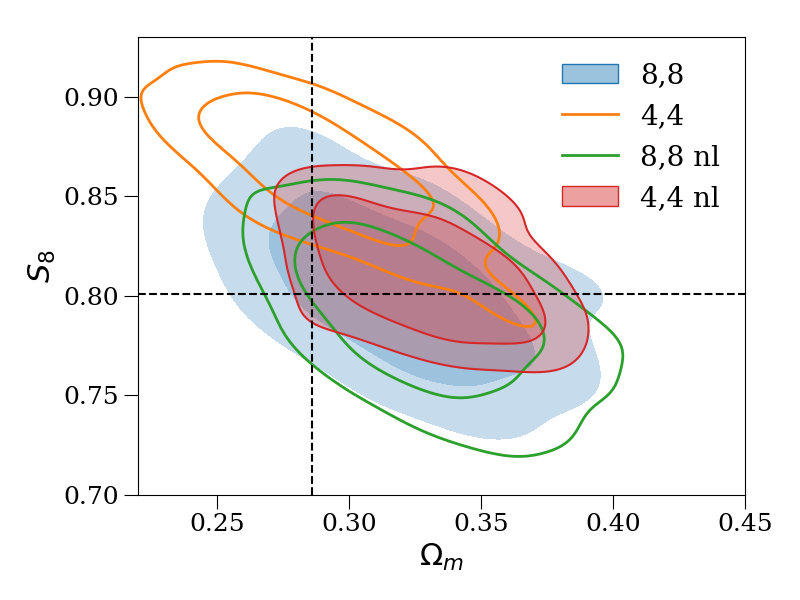
\includegraphics[width=\columnwidth]{figs/buzzard_lcdm_om-s8.png}
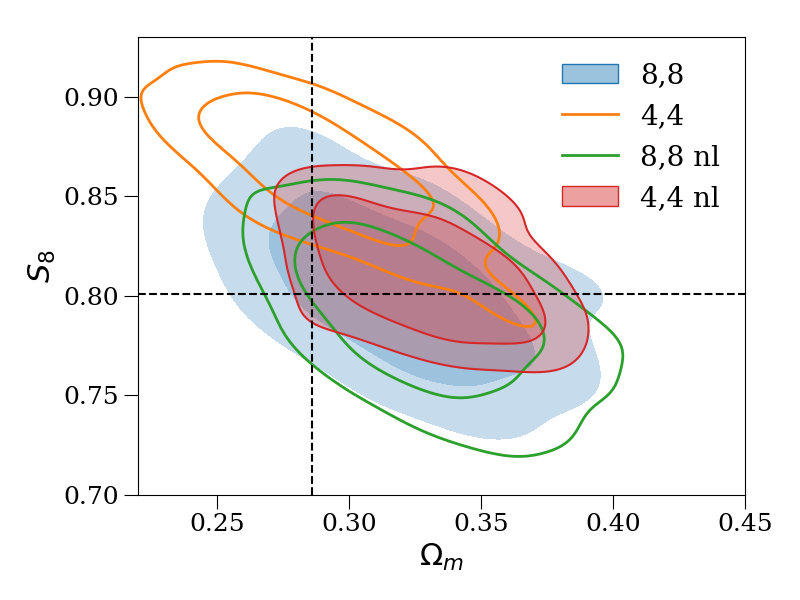
\includegraphics[width=\columnwidth]{figs/buzzard_lcdm_om-s8.png}
\caption[]{\lcdm\ Buzzard constraints }
\label{fig:color_ims}
\end{figure*}

In \fig{fig:bcc_des_lcdm} we show the constraints on $\Omega_m$ and $S_8$ from the mean (over all N realizations) Buzzard 2x2pt measurements, with cosmological parameter priors set I (i.e. wide, ~uninformative priors) in the top panels, and set II in the bottom panels. We show constraints with two sets of scale cuts: 4,4 (left panels) and 8,8 (right panels). In each panel we show constraints for all galaxy bias models (i)-(iv). Comment on which of the options give unbiased cosmology. 

\SP{
\begin{itemize}
    \item \textbf{\textit{Figure}} Linear bias: Based on results on simulated likelihood test, show the cosmology constraints using linear bias model on N-buzzard simulations. 
    \item \textbf{\textit{Figure}} Non-linear bias : Show the $\Omega_m - S_8$ constraints on few scale cuts motivated by the 3D tests. 
\end{itemize}
}


\subsubsection{\wcdm\ with Planck}

\begin{figure*}
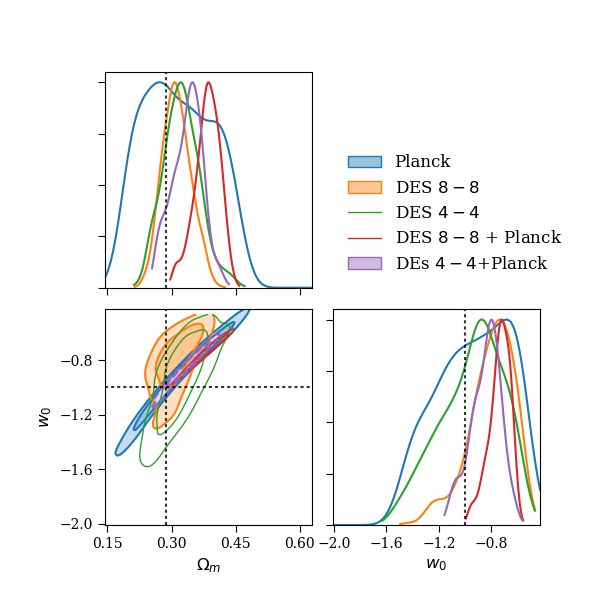
\includegraphics[width=\columnwidth]{figs/buzzard_wcdm_lin_om-w.png}
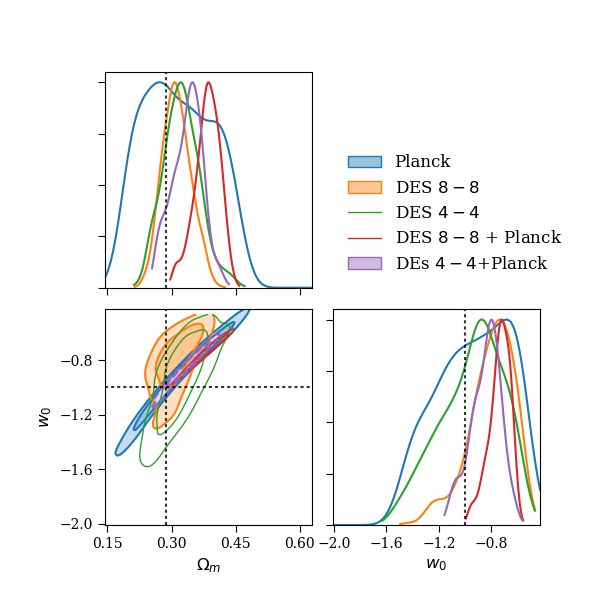
\includegraphics[width=\columnwidth]{figs/buzzard_wcdm_lin_om-w.png}
\caption[]{\wcdm\ Buzzard constraints, linear bias (left panel), non-linear bias (right-panel)}
\label{fig:color_ims}
\end{figure*}

In \fig{fig:bcc_des_wcdm} we show the constraints on $\Omega_m$ and $w$ from the Buzzard 2x2pt measurements, and also simualted Planck CMB data (simulated at the Buzzard cosmology). We use only cosmological prior set I here (but now with free $w$). There'll be a plot for each choice bias model.

Also validate bias modelling choices at fixed cosmology?

\SP{
\begin{itemize}
    \item \textbf{\textit{Figure}} Linear bias: Based on results on simulated likelihood test, show the cosmology constraints using linear bias model on N-buzzard simulations. 
    \item \textbf{\textit{Figure}} Non-linear bias : Show the $\Omega_m - S_8$ constraints on few scale cuts motivated by the 3D tests. 
\end{itemize}
}


\section{Results}

\subsection{DES-only constraints}

Compare DES-only constraints for the three or four analysis variations. Hopefully they agree. Compare performance of different models and present fiducial constraint.

\SP{\begin{itemize}
    \item \textbf{\textit{Figure}} Compare the 1x2pt, 2x2pt and 3x2pt constraints at the 3x2pt defined scale cuts for $\Lambda$CDM. Explain the loss of constraining power in 2x2pt compared to 3x2pt due to PM. Show for both linear bias and non-linear bias. 
\end{itemize}
}

\subsection{Consistency with external datasets}

\subsection{DES+external constraints}

Cosmology and galaxy bias constraints from DES+external. Again compare performance of different analysis choices. Compare bias constraints with some theoretical expectations.

\section*{Acknowledgements}

The Acknowledgements section is not numbered. Here you can thank helpful
colleagues, acknowledge funding agencies, telescopes and facilities used etc.
Try to keep it short.

%%%%%%%%%%%%%%%%%%%%%%%%%%%%%%%%%%%%%%%%%%%%%%%%%%

%%%%%%%%%%%%%%%%%%%% REFERENCES %%%%%%%%%%%%%%%%%%

% The best way to enter references is to use BibTeX:

\bibliographystyle{mnras}
\bibliography{ref} % if your bibtex file is called example.bib


% Alternatively you could enter them by hand, like this:
% This method is tedious and prone to error if you have lots of references
% \begin{thebibliography}{99}
% \bibitem[\protect\citeauthoryear{Author}{2012}]{Author2012}
% Author A.~N., 2013, Journal of Improbable Astronomy, 1, 1
% \bibitem[\protect\citeauthoryear{Others}{2013}]{Others2013}
% Others S., 2012, Journal of Interesting Stuff, 17, 198
% \end{thebibliography}

%%%%%%%%%%%%%%%%%%%%%%%%%%%%%%%%%%%%%%%%%%%%%%%%%%

%%%%%%%%%%%%%%%%% APPENDICES %%%%%%%%%%%%%%%%%%%%%

\appendix

\section{Some extra material}

If you want to present additional material which would interrupt the flow of the main paper,
it can be placed in an Appendix which appears after the list of references.

%%%%%%%%%%%%%%%%%%%%%%%%%%%%%%%%%%%%%%%%%%%%%%%%%%


% Don't change these lines
\bsp	% typesetting comment
\label{lastpage}

% \bibliographystyle{apsrev4-1}
% \bibliography{ref} 

\end{document}

% End of mnras_template.tex